\section{Entrenamiento con Salmons}
% TODO Corrección [14]: Reubicar el análisis comparativo de métricas (mAP, F1, efectos exportación) al nuevo Capítulo 4 (Validación).
Esta sección detalla el proceso de entrenamiento de modelos utilizando la base de datos Salmons. Similar al entrenamiento con Deepfish, se emplearon modelos pre-entrenados con COCO, disponibles en la plataforma Ultralytics, y se ajustaron mediante re-entrenamiento.

\subsection{Entrenamiento inicial}
Idem al caso con Deepfish, este entrenamiento busca establecer una línea base para encaminar los entrenamientos posteriores con búsqueda de hiperparámetros y optimización. Se realizan exactamente los mismos entrenamientos que en la sección \ref{sec:entrenamientoDeepfish}, pero utilizando la base de datos Salmons y con diferentes tamaños de lote, debido a que este conjunto de datos es considerablemente más grande. Para los modelos \textit{n}, \textit{s} y \textit{m} se usó \textit{batch size} 8, para modelos \textit{l} y \textit{c} se usó 6 y para modelos \textit{x} y \textit{e} se usó 4. En total se realizaron 48 entrenamientos.

El análisis es idéntico al de Deepfish, por lo que solo se resumen los resultados más relevantes.
% TODO Corrección [12] [DONE]: Corregir acento "idéntico".

\subsubsection{Efecto del tamaño del modelo}
Igual que con Deepfish, los modelos más pequeños (n, s) mostraron un rendimiento inferior comparandose con modelos más grandes. Sin embargo, esta mejora se estabiliza en modelos medianos y no hay mejoras significativas al usar otros más grandes.

\begin{figure}[htbp]
  \centering
  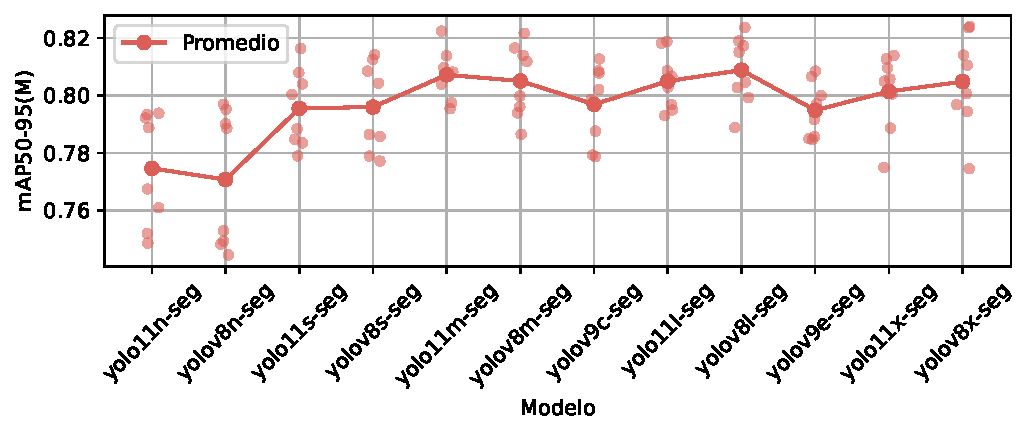
\includegraphics[width=0.9\textwidth]{figures/validation/Salmons-sizeComparison-YOLO-mAP50-95(M).pdf}
  \caption[Puntaje mAP@50-95 en Salmons, por modelo]{Puntaje mAP@50-95 en Salmons, por modelo.}
  \label{fig:salmons_yolo_size_comparison}
\end{figure}

Esto sugiere que para Salmons no hay ventaja considerable en utilizar los modelos más grandes.

\subsubsection{Efecto del Transfer Learning}

Similar a los entrenamientos con Deepfish, el uso de TL mostró un peor rendimiento para la métrica mAP@50-95 en la mayoría de los casos (fig. \ref{fig:salmons_yolo_transfer_Learning_comparison}). Sin embargo, en este caso la caída en rendimiento es más pronunciada y ocurre también en F1 y mAP@50 (aunque no se muestren en la figura). Similarmente, la caida en rendimiento se acrecenta al exportar a TensorRT-INT8 (fig. \ref{fig:salmons_yolo_dataset_factor_mejora_by_format}).

\begin{figure}[htbp]
  \centering
  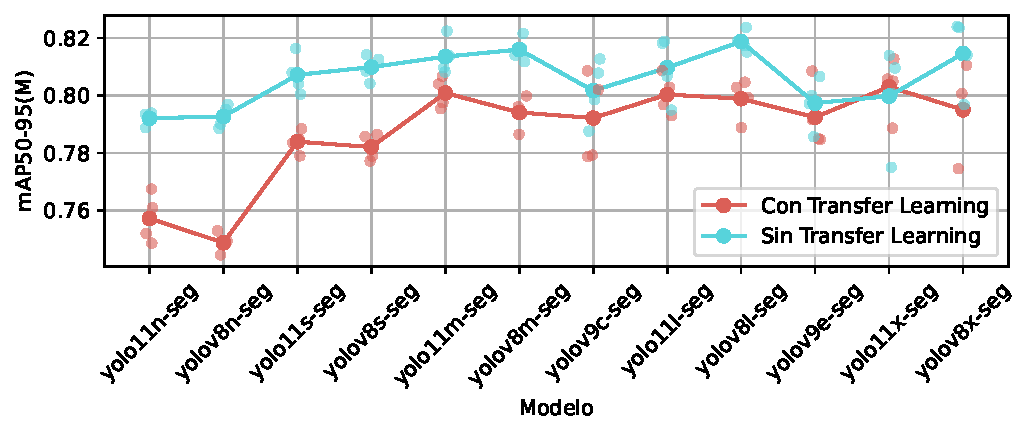
\includegraphics[width=0.9\textwidth]{figures/validation/Salmons-TransferLearningComparison-YOLO-mAP50-95(M).pdf}
  \caption[Comparación de métricas por modelo YOLO en Salmons con y sin Transfer Learning]{Comparación de rendimiento mAP@50-95 por modelo YOLO en Salmons con y sin Transfer Learning.}
  \label{fig:salmons_yolo_transfer_Learning_comparison}
\end{figure}

\subsubsection{Efecto del optimizador}
Similar a como ocurre con Deepfish, SGD supera marginalmente a AdamW en la mayoría de los casos (fig. \ref{fig:salmons_yolo_optimizer_map50_95}) siendo un 1.5\% mejor en mAP50-95 y 2.4\% mejor con cuantización INT8 (tablas \ref{tab:salmons_factorMejora_optimizer_by_model} y \ref{tab:salmons_factorMejora_optimizer_by_format}). Para esta base de datos no se dieron casos de entrenamientos que no convergieran con AdamW, por eso no hay análisis con \textit{outliers}, pero en general SGD mostró un mejor desempeño a pesar de ello.

\begin{table}[htbp]
\centering
\caption[Factor de mejora entre SGD y AdamW en Salmons, por modelo]{Factor de mejora promedios entre SGD y AdamW, por modelo YOLO. Valores mayores a 1 indican que SGD supera a AdamW.}
\label{tab:salmons_factorMejora_optimizer_by_model}
\begin{tabular}{|r|r|r|r|}
\hline
\multicolumn{1}{|c|}{\textbf{F1\_score(M)}} & \multicolumn{1}{c|}{\textbf{mAP50(M)}} & \multicolumn{1}{c|}{\textbf{mAP50-95(M)}} & \multicolumn{1}{c|}{\textbf{Model}} \\ \hline
1.003387 & 1.007258 & 1.007882 & yolov8n-seg \\ \hline
1.003012 & 1.002322 & 1.006601 & yolov8s-seg \\ \hline
0.998518 & 0.997383 & 1.011763 & yolov8m-seg \\ \hline
1.007857 & 0.996747 & 1.013573 & yolov8l-seg \\ \hline
1.009566 & 1.006145 & 1.030187 & yolov8x-seg \\ \hline
1.007747 & 1.007785 & 1.028812 & yolov9c-seg \\ \hline
1.008252 & 1.008075 & 1.022180 & yolov9e-seg \\ \hline
0.993766 & 0.999840 & 1.004929 & yolo11n-seg \\ \hline
1.011274 & 1.005820 & 1.014746 & yolo11s-seg \\ \hline
0.998538 & 0.998664 & 1.007837 & yolo11m-seg \\ \hline
0.998261 & 1.002217 & 1.015270 & yolo11l-seg \\ \hline
0.998836 & 1.000598 & 1.022320 & yolo11x-seg \\ \hline
1.003251 & 1.002738 & 1.015508 & Promedio \\ \hline
\end{tabular}
\end{table}

\begin{figure}[htbp]
  \centering
  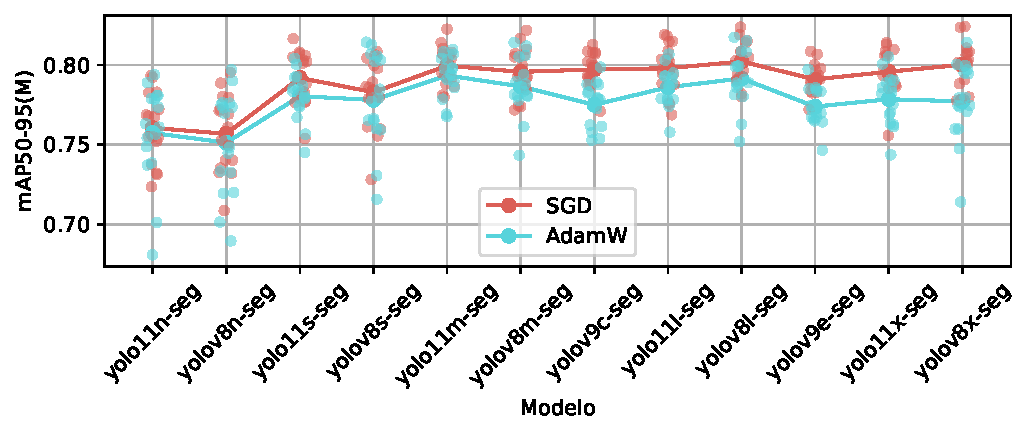
\includegraphics[width=0.9\textwidth]{figures/validation/Salmons-OptimizerComparison-YOLO-mAP50-95(M).pdf}
  \caption[Puntaje mAP@50-95 por modelo YOLO en Salmons (AdamW vs SGD)]{Comparación del puntaje mAP@50-95 para distintos modelos YOLO en Salmons, utilizando los optimizadores AdamW y SGD.}
  \label{fig:salmons_yolo_optimizer_map50_95}
\end{figure}


\newpage
\subsubsection{Efecto de las imágenes de fondo (Full vs ``LO'')}
A diferencia de Deepfish, en Salmons no se observaron diferencias significativas promedio entre entrenar con imágenes de fondo (Full) o sin ellas (``LO'') (tabla \ref{tab:salmons_mejoraRelativa_model} y fig. \ref{fig:salmons_yolo_dataset_comparison}). En promedio incluir imágenes de fondo empeora el rendimiento en 0.12\% en mAP@50-95. Similar a Deepfish, esta diferencia aumenta al exportar a TensorRT-INT8, decayendo en hasta un 3\% su rendimiento (fig. \ref{fig:salmons_yolo_transfer_learning_factor_mejora_by_format}).
% TODO Corrección [12] [DONE]: Cambiar "imagenes" -> "imágenes" (dos veces).

Por paradojico que parezca, este comportamiento puede deberse a que al ser Salmons una base de datos más grande, el modelo aprende a generalizar mejor sin necesidad de imágenes de fondo e incluiras solo ``diluye'' la relevancia de cada imagen en el entrenamiento, afectando su aprendizaje. Esto empeora aún más al exportarse con TensorRT con cuantización numérica pues simplificar el modelo implica la pérdida de información en el espacio latente (pesos del modelo), y si estos ya están muy ``diluidos'' o distribuidos homogeneamente, se vuelve incluso más díficil caracterizar objetos de interes y distinguirlos del fondo.

Otra alternativa se haya en cómo está definida la base de datos de validación. Al poseer pocas imágenes sin instancias de peces o con contextos complejos que se beneficien de distinguir salmones de no salmones, el modelo no es capaz de validar correctamente su aprendizaje y pareciera que es peor, cuando en la práctica podría no serlo.
% TODO Corrección [12] [DONE]: Cambiar "imagenes" -> "imágenes" y "en como" -> "en cómo".

\begin{table}[htbp]
\centering
\caption[Mejora relativa del uso de imágenes de fondo en Salmons, por modelo]{Mejora relativa del uso de imágenes de fondo en Salmons, por modelo. Valores mayores a 1 indican que la versión completa supera a ``LO''.}
\label{tab:salmons_mejoraRelativa_model}
\begin{tabular}{|r|r|r|r|}
\hline
\multicolumn{1}{|c|}{\textbf{F1\_score(M)}} & \multicolumn{1}{c|}{\textbf{mAP50(M)}} & \multicolumn{1}{c|}{\textbf{mAP50-95(M)}} & \multicolumn{1}{c|}{\textbf{Model}} \\ \hline
1.005496 & 1.006961 & 1.003863 & yolo11n-seg \\ \hline
1.003430 & 1.010441 & 1.011589 & yolov8n-seg \\ \hline
0.990748 & 0.995516 & 0.995070 & yolo11s-seg \\ \hline
1.007440 & 1.007474 & 1.003930 & yolov8s-seg \\ \hline
0.997610 & 1.009629 & 1.003682 & yolo11m-seg \\ \hline
1.008691 & 1.004680 & 1.003225 & yolov8m-seg \\ \hline
0.998423 & 1.001868 & 0.994404 & yolov9c-seg \\ \hline
1.006509 & 1.005648 & 0.997777 & yolo11l-seg \\ \hline
1.004114 & 1.004073 & 1.000431 & yolov8l-seg \\ \hline
0.988721 & 1.001341 & 0.992500 & yolov9e-seg \\ \hline
0.993250 & 0.999378 & 0.986374 & yolo11x-seg \\ \hline
1.002447 & 1.006548 & 0.992197 & yolov8x-seg \\ \hline
1.000573 & 1.004463 & 0.998753 & Promedio \\ \hline
\end{tabular}
\end{table}

\begin{figure}[htb]
  \centering
  \begin{subfigure}[b]{\textwidth}
    \centering
    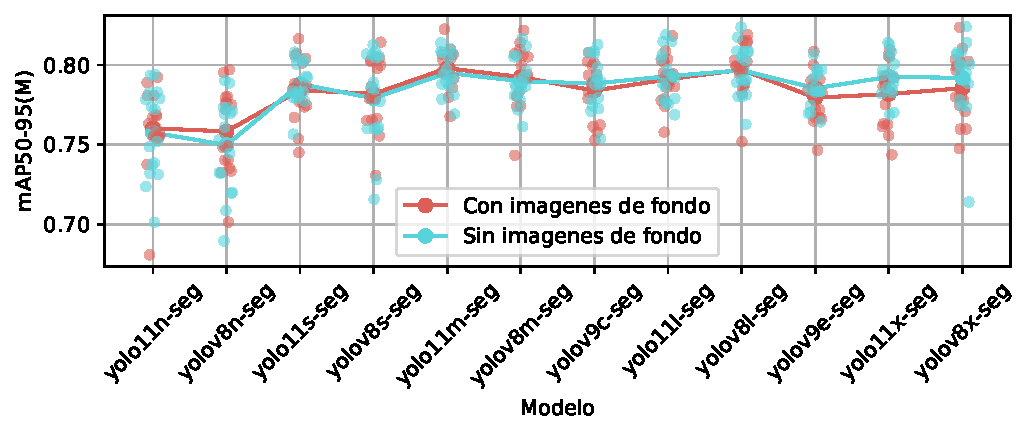
\includegraphics[width=0.9\textwidth]{figures/validation/Salmons-DatasetComparison-YOLO-mAP50-95(M).pdf}
    \caption{Comparación del puntaje mAP@50-95 entre los \textit{datasets} Full y ``LO'' de Salmons.}
    \label{fig:salmons_yolo_dataset_comparison_map50_95}
  \end{subfigure}

  \begin{subfigure}[b]{\textwidth}
    \centering
    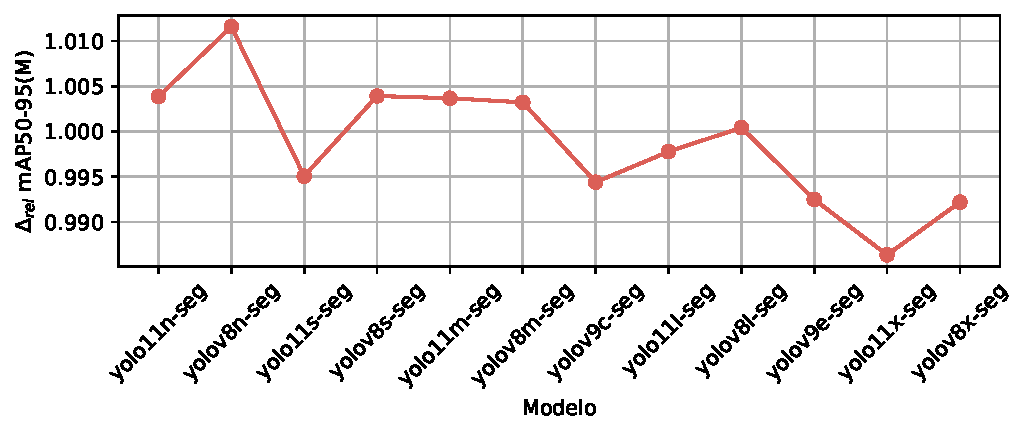
\includegraphics[width=0.9\textwidth]{figures/validation/Salmons-DatasetFactorMejora-YOLO-mAP50-95(M).pdf}
    \caption{Factor de mejora promedio entre los \textit{datasets} Full y ``LO'' de Salmons, por modelo. Valores mayores a 1 indican que la versión Full supera a ``LO''.}
    \label{fig:salmons_yolo_dataset_factor_mejora_by_model}
  \end{subfigure}

  \caption[Comparación del rendimiento entre los \textit{datasets} Full y ``LO'' de Salmons]{Comparación del rendimiento entre los \textit{datasets} Full y ``LO'' de Salmons, por modelo.}
  \label{fig:salmons_yolo_dataset_comparison}
\end{figure}

\subsubsection{Efecto del formato de exportación}
Igual que con Deepfish se observa que la exportación a TensorRT en precisión FP32 y FP16 tiene un impacto mínimo en el rendimiento del modelo ($\sim$1.41\% en mAP50 y $\sim$1.57\% en mAP50-95), y la cuantización a INT8 resulta en una degradación más significativa ($\sim$3\% en mAP50 y $\sim$3.6\% en mAP50-95) (tabla \ref{tab:salmons_mejoraRelativaPromedio_format} y fig. \ref{fig:salmons_yolo_format_comparison}).

A diferencia de Deepfish, la degradación en rendimiento al exportar a TensorRT-INT8 es menor, pero esto ocurre porque los modelos más pequeños (n, s) no sufren una caída tan pronunciada en rendimiento al exportar a INT8, a diferencia de Deepfish donde estos modelos sufrieron caídas de hasta un 50\% en mAP@50-95 (fig. \ref{fig:deepfish_yolo_format_comparison}). Puede que al ser Salmons más grande los modelos pequeños si alcanzan a aprender correctamente la caracterización de sus clases.

El incremento en velocidad de inferencia depende del formato de exportación y modelo, no tanto del \textit{dataset}, por ende los resultados son equivalentes a los obtenidos con Deepfish.

\begin{table}[htbp]
\centering
\caption[Mejora relativa de exportar con TensorRT con diferentes precisiones en Salmons]{Mejora relativa de exportar con TensorRT con diferentes precisiones en Salmons. Valores menores a 1 indican caída de rendimiento de Pytorch a TensorRT, para tiempos de inferencia es al revés.}
\label{tab:salmons_mejoraRelativaPromedio_format}
\begin{tabular}{|r|r|r|r|r|}
\hline
\multicolumn{1}{|c|}{\textbf{F1\_score(M)}} & \multicolumn{1}{c|}{\textbf{mAP50(M)}} & \multicolumn{1}{c|}{\textbf{mAP50-95(M)}} & \multicolumn{1}{c|}{\textbf{inference}} & \multicolumn{1}{c|}{\textbf{Format}} \\ \hline
0.980275 & 0.985921 & 0.983856 & 0.899806 & TensorRT-F32 \\ \hline
0.980396 & 0.985972 & 0.984756 & 0.332805 & TensorRT-F16 \\ \hline
0.957552 & 0.969573 & 0.963565 & 0.239950 & TensorRT-INT8 \\ \hline
\end{tabular}
\end{table}

\begin{figure}[htbp]
\begin{center}
    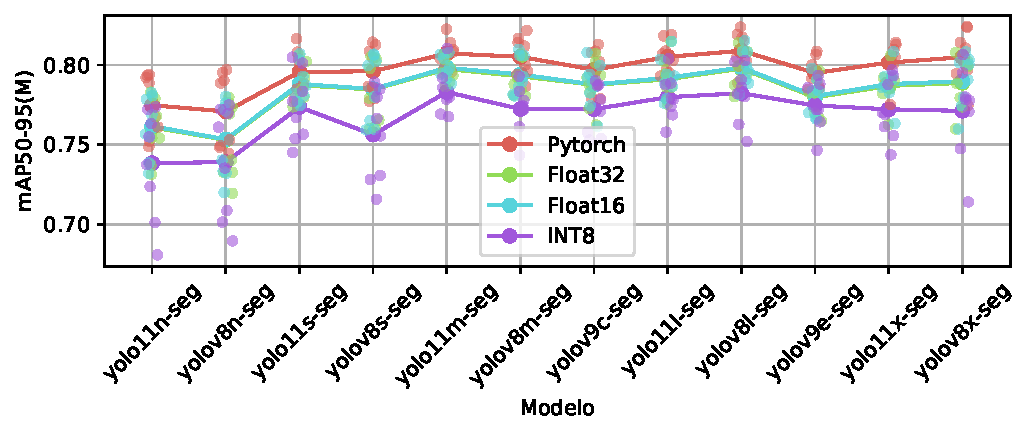
\includegraphics[width=0.9\textwidth]{figures/validation/Salmons-FormatComparison-YOLO-mAP50-95(M).pdf}
    \caption[Comparación del rendimiento entre formatos de exportación en Salmons]{Comparación del rendimiento entre los formatos de exportación (PyTorch vs TensorRT) en Salmons.}
    \label{fig:salmons_yolo_format_comparison}
\end{center}
\end{figure}

De manera similar, la caida en rendimiento al optimizar el modelo se incrementa con ciertas configuraciones, en este caso siendo el uso del optimizador AdamW, \textit{Transfer Learning} y la inclusión de imágenes de fondo (tabla \ref{tab:salmons_factorMejora_optimizer_by_format} y figs. \ref{fig:salmons_yolo_transfer_learning_factor_mejora_by_format} y \ref{fig:salmons_yolo_dataset_factor_mejora_by_format}). Similar a Deepfish, estos efectos sugieren que estas prácticas pueden limitar la capacidad del modelo para aprender adecuadamente a lo largo de todos sus pesos, mas hay que ser cauteloso al interpretar estos resultados especialmente en el caso de la inclusión de imágenes de fondo, ya que ocurre lo contrario a lo que se esperaría y esto debe ser estudiado más a fondo e interpretado con cautela.
% TODO Corrección [12] [DONE]: Sustituir "tomado con pinzas" por "interpretado con cautela".

\begin{table}[htbp]
\centering
\caption[Factor de mejora entre SGD y AdamW en Salmons, por formato]{Factor de mejora promedios entre SGD y AdamW, por formato de exportación. Valores mayores a 1 indican que SGD supera a AdamW.}
\label{tab:salmons_factorMejora_optimizer_by_format}
\begin{tabular}{|r|r|r|r|}
\hline
\multicolumn{1}{|c|}{\textbf{F1\_score(M)}} & \multicolumn{1}{c|}{\textbf{mAP50(M)}} & \multicolumn{1}{c|}{\textbf{mAP50-95(M)}} & \multicolumn{1}{c|}{\textbf{Format}} \\ \hline
1.000905 & 1.000132 & 1.012125 & Pytorch \\ \hline
1.001709 & 1.002062 & 1.012591 & TensorRT-F32 \\ \hline
1.001856 & 1.002117 & 1.012900 & TensorRT-F16 \\ \hline
1.008536 & 1.006641 & 1.024416 & TensorRT-INT8 \\ \hline
1.003251 & 1.002738 & 1.015508 & Promedio \\ \hline
\end{tabular}
\end{table}

\begin{figure}[htbp]
  \centering
  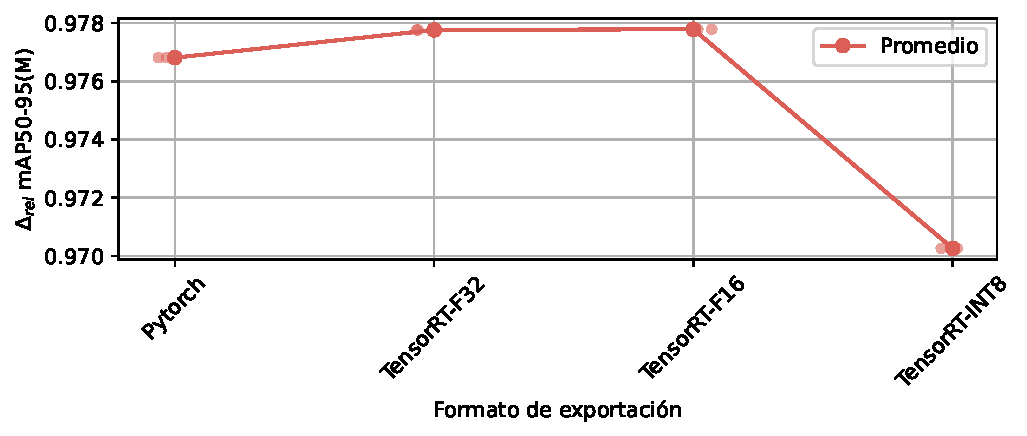
\includegraphics[width=0.9\textwidth]{figures/validation/Salmons-TransferLearningFactorMejora-Format-mAP50-95(M).pdf}
  \caption[Factor de mejora de usar TransferLearning en Salmons, por formato]{Factor de mejora de usar TransferLearning en Salmons, por formato de exportación. Valores menores a 1 indican caída en rendimiento al usar Transfer Learning.}
  \label{fig:salmons_yolo_transfer_learning_factor_mejora_by_format}
\end{figure}

\begin{figure}[htbp]
  \centering
  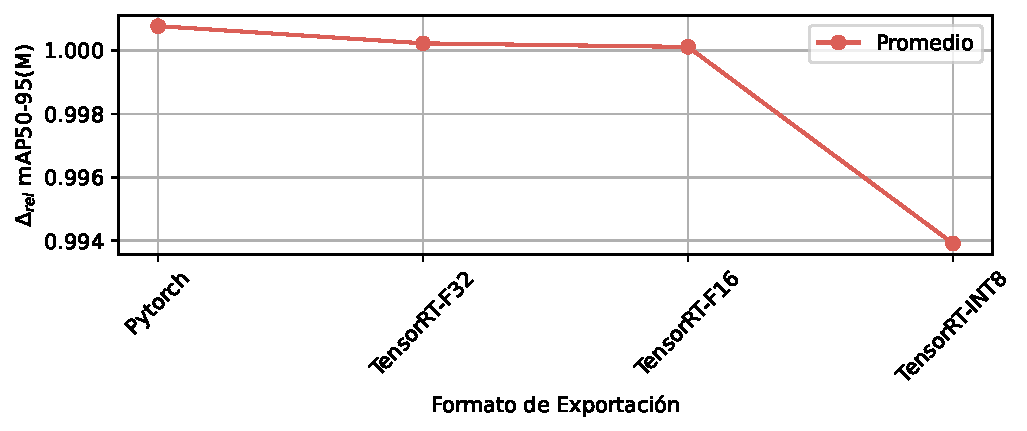
\includegraphics[width=0.9\textwidth]{figures/validation/Salmons-DatasetFactorMejora-Format-mAP50-95(M).pdf}
  \caption[Factor de mejora entre los \textit{datasets} Full y ``LO'' de Salmons, por formato]{Factor de mejora entre los \textit{datasets} Full y ``LO'' de Salmons, por formato de exportación. Valores mayores a 1 indican que la versión Full supera a ``LO''.}
  \label{fig:salmons_yolo_dataset_factor_mejora_by_format}
\end{figure}

\subsection{Búsqueda de hiperparámetros y entrenamiento final}
Idem al caso con Deepfish, se realizó una búsqueda de hiperparámetros utilizando la herramienta Raytune en Ultralytics con el mismo espacio de búsqueda (tabla \ref{tab:search_space}), para finalmente re-entrenar los modelos con los mejores hiperparámetros encontrados.

\begin{itemize}
    \setlength{\itemsep}{0pt}%
    %\setlength{\parskip}{0pt}%
    %\setlength{\parsep}{0pt}%
    \item \textbf{Transfer Learning}: dado a ser inferior en todas las métricas, se omite el uso de \textit{Transfer Learning} y se opta por entrenar el modelo completo.
    \item \textbf{Optimizador}: igual que con Deepfish, se opta por usar SGD.
    \item \textbf{Versión del dataset}: si bien los resultados parecen indicar que la incorporación de imágenes de fondo afecta negativamente el rendimiento del modelo, este efecto no es concluyente y puede deberse a otros factores como la calidad de la base de datos de validación o una carencia intrinseca de definir bien instancias ``correctas'' de salmones en el \textit{dataset} ---esto se discute más adelante. Por ende, se opta por entrenar con la versión completa por un tema de buena práctica.
    \item \textbf{Modelos}: ante la falta de evidencia de que los modelos más grandes aporten mejoras significativas, se opta por entrenar los modelos medianos YOLOv8m, YOLOv8l, YOLOv9c, YOLO11m y YOLO11l. Esto es relevante pues los modelos más grandes requieren más recursos computacionales, tiempo de entrenamiento y sufren de mayor latencia en inferencia, lo cual es contraproducente para aplicaciones en tiempo real.
\end{itemize}

Debido a que Salmons es una base de datos más grande, se decide que es mejor realizar dos entrenamientos de 50 épocas en vez de un único de 80. Para ello se realizarán 50 entrenamientos por modelo, cada uno de 50 épocas, con tamaños de lote 8 para los modelos YOLOv8m y YOLO11m y 6 para los otros. Una vez terminada la primera ronda de búsqueda de hiperparámetros, se selecciona el mejor caso obtenido por cada modelo (mejor mAP@50-95) y se realiza una segunda ronda de búsqueda. Finalmente se utiliza el mejor caso de cada modelo. En total se realizan 500 entrenamientos y las métricas de validación resultantes se muestran en la tabla \ref{tab:salmons_resultados_finales}.

Esta vez se incluyen los resultados de exportar a TensorRT-F16 además de TensorRT-INT8, esto porque es capaz de reducir el tiempo de inferencia a la mitad sin comprometer tanto el rendimiento del modelo, lo que lo hace atractivo para este caso de uso.

\subsubsection{Ejemplos de segmentación}
A continuación se muestran ejemplos de segmentación obtenidos con los modelos entrenados en Salmons (fig. \ref{fig:salmons_segmentation_examples}). Para estos ejemplos se usó el modelo YOLOv8l-seg.

\begin{figure}[htbp]
\centering
%\setlength{\tabcolsep}{4pt} % Espaciado horizontal entre columnas
%\renewcommand{\arraystretch}{1.0} % Espaciado vertical entre filas
\begin{tabular}{ccc}
    % ====== Ejemplo 1 ======
    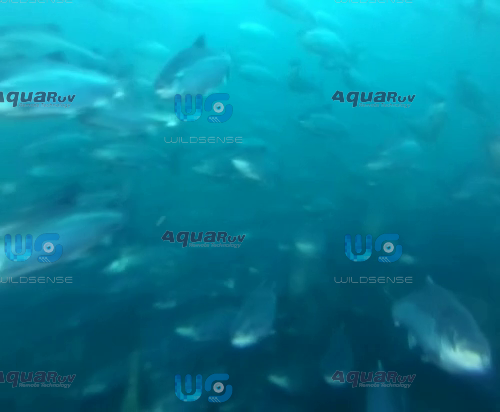
\includegraphics[width=0.25\textwidth]{figures/results/salmones/original/Seguimiento_1_000219.png} &
    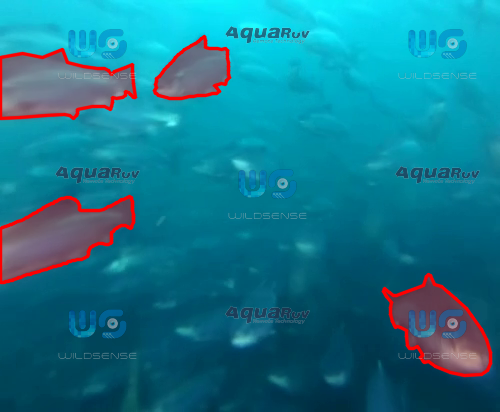
\includegraphics[width=0.25\textwidth]{figures/results/salmones/painted/Seguimiento_1_000219.png} &
    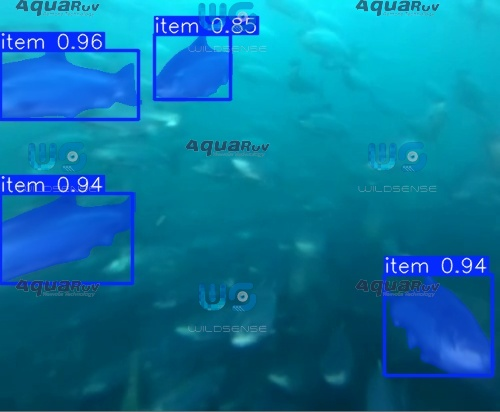
\includegraphics[width=0.25\textwidth]{figures/results/salmones/predict/Seguimiento_1_000219.jpg} \\

    % ====== Ejemplo 2 ======
    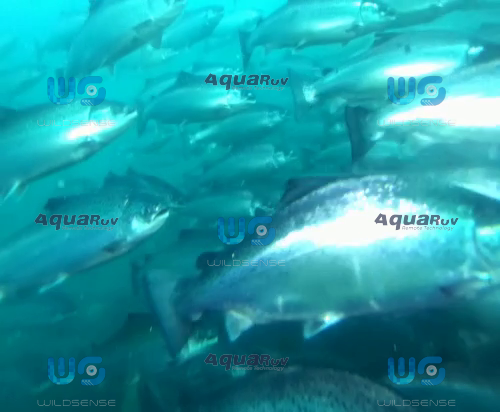
\includegraphics[width=0.25\textwidth]{figures/results/salmones/original/Seguimiento_2_000033.png} &
    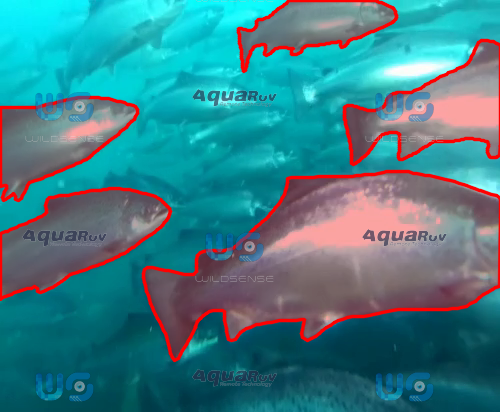
\includegraphics[width=0.25\textwidth]{figures/results/salmones/painted/Seguimiento_2_000033.png} &
    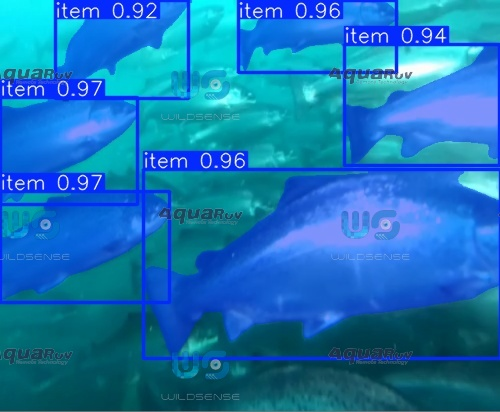
\includegraphics[width=0.25\textwidth]{figures/results/salmones/predict/Seguimiento_2_000033.jpg} \\

    % ====== Ejemplo 3 ======
    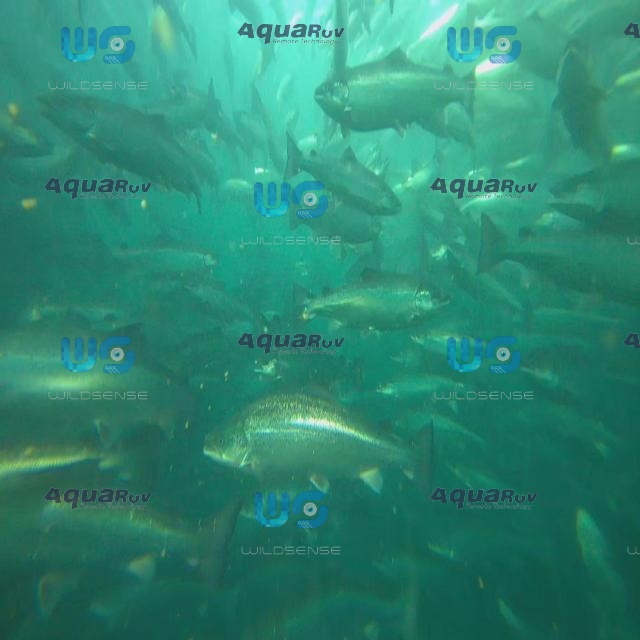
\includegraphics[width=0.25\textwidth]{figures/results/salmones/original/741_png_jpg.rf.836cc3dba57ee593e9b4b5a1a61f099d.jpg} &
    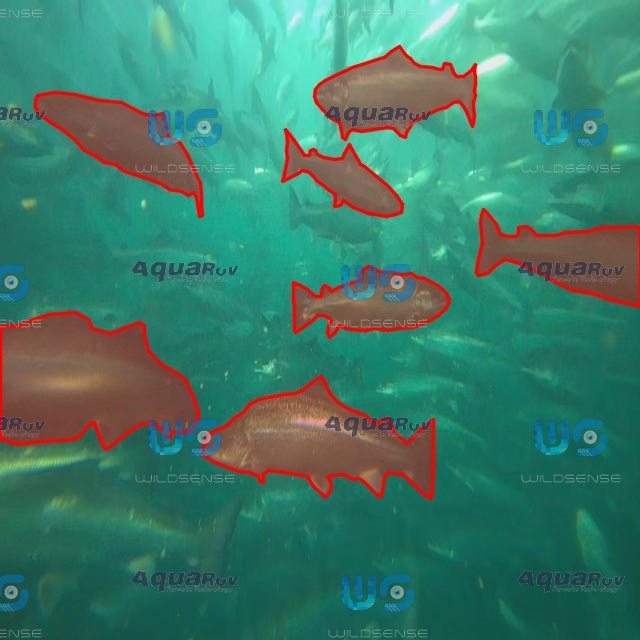
\includegraphics[width=0.25\textwidth]{figures/results/salmones/painted/741_png_jpg.rf.836cc3dba57ee593e9b4b5a1a61f099d.jpg} &
    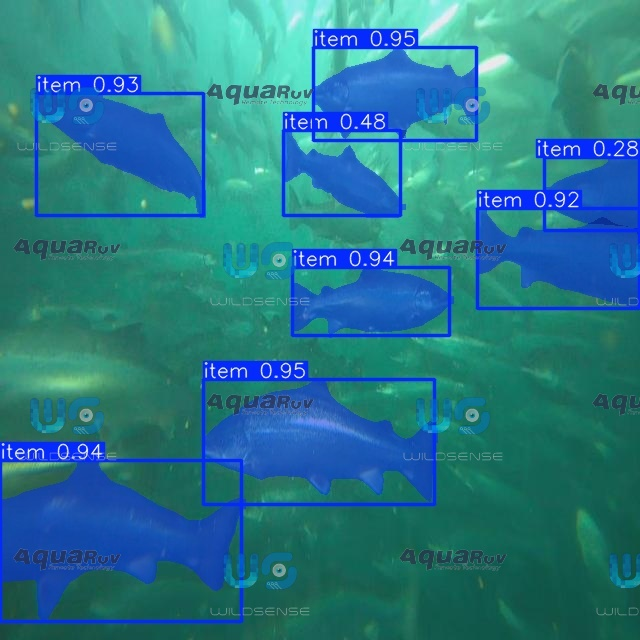
\includegraphics[width=0.25\textwidth]{figures/results/salmones/predict/741_png_jpg.rf.836cc3dba57ee593e9b4b5a1a61f099d.jpg} \\

    % ====== Ejemplo 4 ======
    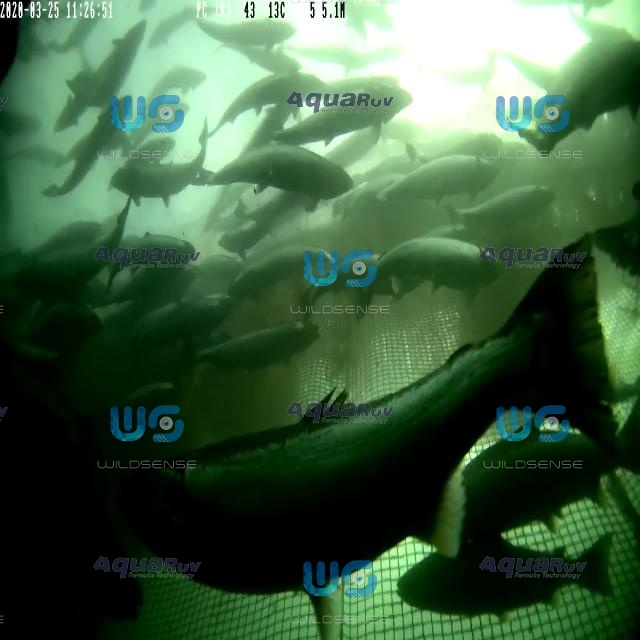
\includegraphics[width=0.25\textwidth]{figures/results/salmones/original/Img3_jpeg.rf.3a846528a9da542cae08a04d32cb2468.jpg} &
    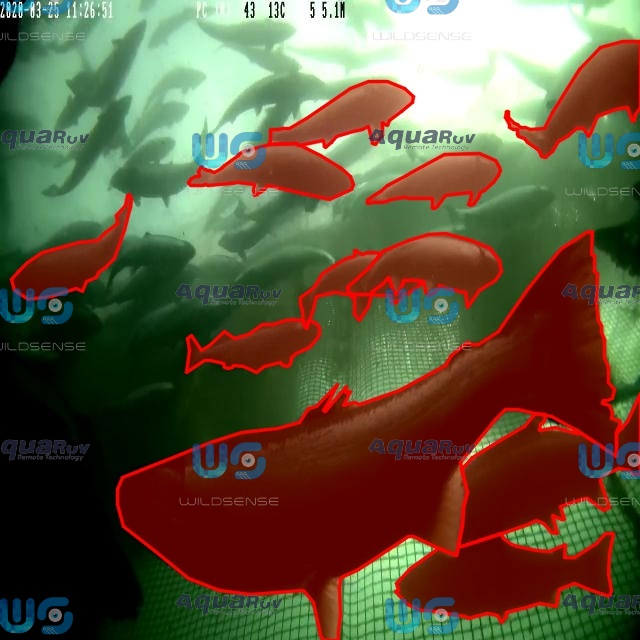
\includegraphics[width=0.25\textwidth]{figures/results/salmones/painted/Img3_jpeg.rf.3a846528a9da542cae08a04d32cb2468.jpg} &
    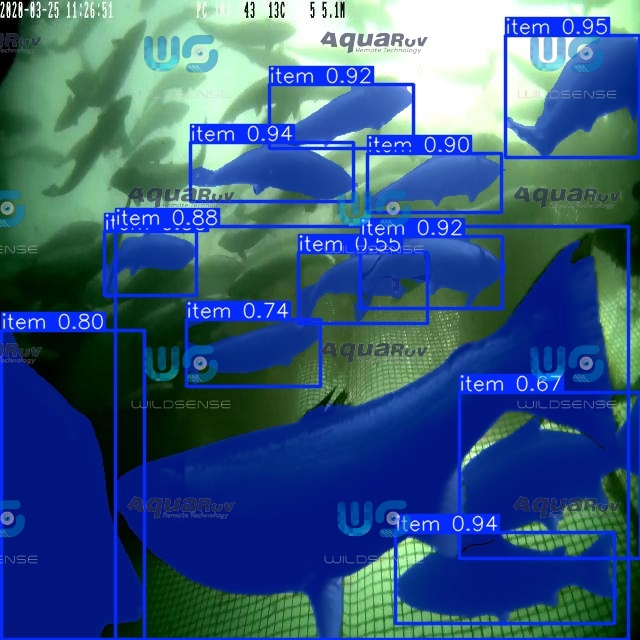
\includegraphics[width=0.25\textwidth]{figures/results/salmones/predict/Img3_jpeg.rf.3a846528a9da542cae08a04d32cb2468.jpg} \\

    % ====== Ejemplo 5 ======
    %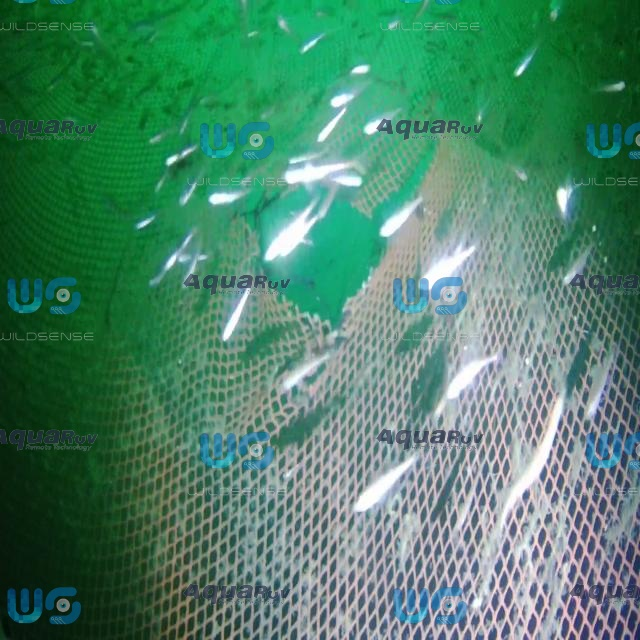
\includegraphics[width=0.2\textwidth]{figures/results/salmones/original/Sep25_270_png.rf.afa3b720cb52b7b4e34639773be3a4b7.jpg} &
    %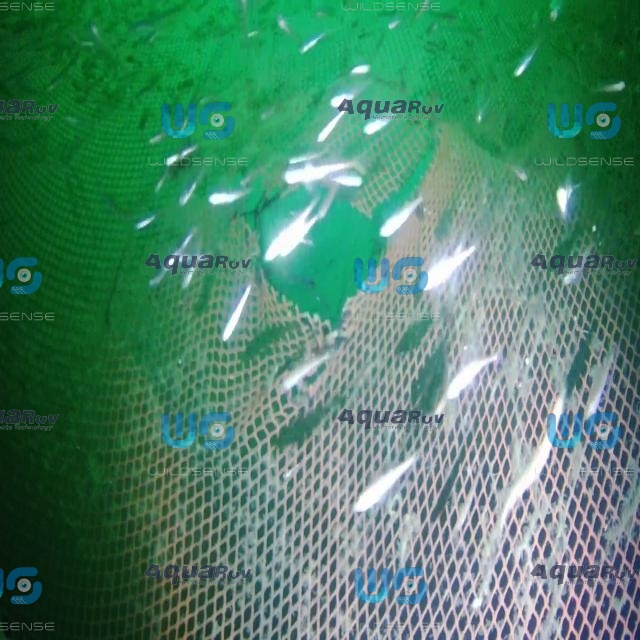
\includegraphics[width=0.2\textwidth]{figures/results/salmones/painted/Sep25_270_png.rf.afa3b720cb52b7b4e34639773be3a4b7.jpg} &
    %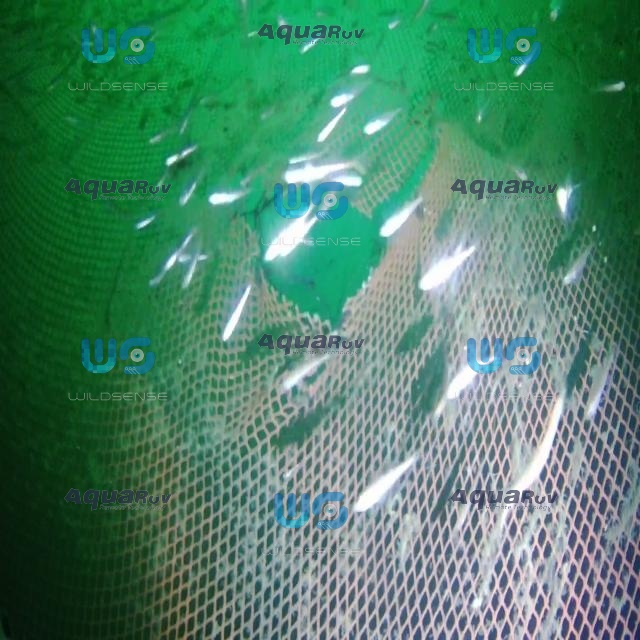
\includegraphics[width=0.2\textwidth]{figures/results/salmones/predict/Sep25_270_png.rf.afa3b720cb52b7b4e34639773be3a4b7.jpg} \\
\end{tabular}
\caption[Ejemplos de segmentación obtenidos en Salmons]{Ejemplos de segmentación obtenidos con el modelo YOLOv8l-seg entrenado en \textit{Salmons}. De izquierda a derecha: imagen original; máscaras etiquetadas (\textit{Ground Truth}) en rojo; predicción del modelo en azul.}
\label{fig:salmons_segmentation_examples}
\end{figure}